% ******************************************************
% A Classic Thesis Style
% An Homage to The Elements of Typographic Style
%
% Copyright (C) 2018 André Miede and Ivo Pletikosić
% ******************************************************
\RequirePackage{silence}
    \WarningFilter{scrreprt}{Usage of this version of package `titlesec'}
    \WarningFilter{scrreprt}{Usage of package `tocloft' together}
    \WarningFilter{titlesec}{Non standard sectioning command}
\documentclass[% TODO: go through these
    twoside,
    openright,
    titlepage,
    numbers=noenddot,
    %1headlines,
    headinclude,
    footinclude,
    cleardoublepage=empty,
    abstract=on,
    BCOR=5mm,
    paper=a4,
    fontsize=11pt
]{scrreprt}

% ******************************************************
% Note: Make all your adjustments in here
% ******************************************************
\PassOptionsToPackage{utf8}{inputenc}
\usepackage{inputenc}

\PassOptionsToPackage{T1}{fontenc}
\usepackage{fontenc}


% ********************************************************************
% 1. Configure classicthesis for your needs here, e.g., remove "drafting" below
% in order to deactivate the time-stamp on the pages
% (see ClassicThesis.pdf for more information):
% ********************************************************************
\PassOptionsToPackage{
    drafting=true,    % print version information on the bottom of the pages
    tocaligned=false, % the left column of the toc will be aligned (no indentation)
    dottedtoc=false,  % page numbers in ToC flushed right
    eulerchapternumbers=true, % use AMS Euler for chapter font (otherwise Palatino)
    linedheaders=false,       % chaper headers will have line above and beneath
    floatperchapter=true,     % numbering per chapter for all floats (i.e., Figure 1.1)
    eulermath=false,  % use awesome Euler fonts for mathematical formulae (only with pdfLaTeX)
    beramono=true,    % toggle a nice monospaced font (w/ bold)
    palatino=true,    % deactivate standard font for loading another one, see the last section at the end of this file for suggestions
    style=classicthesis % classicthesis, arsclassica
}{classicthesis}


% ********************************************************************
% 2. Personal data and user ad-hoc commands (insert your own data here)
% ********************************************************************
\newcommand{\myTitle}{Quantum Circuit Compilation From The Ground Up\xspace}
\newcommand{\mySubtitle}{\xspace}
\newcommand{\myDegree}{Master of Mathematics (MMath)\xspace}
\newcommand{\myName}{Nathaniel Stemen\xspace}
% \newcommand{\myProf}{Someone else TODO\xspace}
\newcommand{\mySupervisor}{Joel Wallman\xspace}
\newcommand{\myFaculty}{Faculty of Mathematics\xspace}
\newcommand{\myDepartment}{Department of Applied Mathematics\xspace}
\newcommand{\myUni}{University of Waterloo\xspace}
\newcommand{\myInst}{Institute for Quantum Computing\xspace}
\newcommand{\myLocation}{Seattle, WA\xspace}
\newcommand{\myTime}{April 2022\xspace}
\newcommand{\myTimeFrame}{September 2020---April 2022}
\newcommand{\myVersion}{\classicthesis}

% ********************************************************************
% Setup, finetuning, and useful commands
% ********************************************************************
\newcommand{\ie}{i.\,e.}
\newcommand{\Ie}{I.\,e.}
\newcommand{\eg}{e.\,g.}
\newcommand{\Eg}{E.\,g.}


% ********************************************************************
% 3. Loading some handy packages
% ********************************************************************

% ********************************************************************
% Packages with options that might require adjustments
% ********************************************************************
\PassOptionsToPackage{american}{babel}
\usepackage{babel}

\usepackage{csquotes}

\PassOptionsToPackage{
    style=alphabetic,
    maxnames=5,
    backref=true
}{biblatex}
\usepackage{biblatex}

\PassOptionsToPackage{fleqn}{amsmath} % float equations towards left side
\usepackage{amsmath}
\newtheorem{theorem}{Theorem}[section]
\newtheorem{definition}[theorem]{Definition}
\newtheorem{example}[theorem]{Example}
\newtheorem{question}[theorem]{Question}

\usepackage{physics}
\usepackage{mathtools}
\usepackage{stmaryrd}
\DeclarePairedDelimiter\dbrackets{\llbracket}{\rrbracket}

% ********************************************************************
% General useful packages
% ********************************************************************
\usepackage{graphicx}
\usepackage{scrhack} % fix warnings when using KOMA with listings package
\usepackage{xspace} % to get the spacing after macros right
\PassOptionsToPackage{printonlyused,smaller}{acronym}
\usepackage{acronym} % TODO change to acro package


% ********************************************************************
% 4. Setup floats: tables, (sub)figures, and captions
% ********************************************************************
\usepackage{tabularx} % better tables: TODO change to booktabs
\setlength{\extrarowheight}{3pt} % increase table row height
\newcommand{\tableheadline}[1]{\multicolumn{1}{l}{\spacedlowsmallcaps{#1}}}
\newcommand{\myfloatalign}{\centering} % to be used with each float for alignment
\usepackage{subfig}


% ********************************************************************
% 5. Setup code listings
% ********************************************************************
\usepackage{listings}
%\lstset{emph={trueIndex,root},emphstyle=\color{BlueViolet}}%\underbar} % for special keywords
\lstset{language=[LaTeX]Tex,%C++,
    morekeywords={PassOptionsToPackage,selectlanguage},
    keywordstyle=\color{RoyalBlue},%\bfseries,
    basicstyle=\small\ttfamily,
    %identifierstyle=\color{NavyBlue},
    commentstyle=\color{Green}\ttfamily,
    stringstyle=\rmfamily,
    numbers=none,%left,%
    numberstyle=\scriptsize,%\tiny
    stepnumber=5,
    numbersep=8pt,
    showstringspaces=false,
    breaklines=true,
    %frameround=ftff,
    %frame=single,
    belowcaptionskip=.75\baselineskip
    %frame=L
}


% ********************************************************************
% 6. Last calls before the bar closes
% ********************************************************************
\usepackage{classicthesis}


% ********************************************************************
% Fine-tune hyperreferences (hyperref should be called last)
% ********************************************************************
\hypersetup{%
    %draft, % hyperref's draft mode, for printing see below
    colorlinks=true, linktocpage=true, pdfstartpage=3, pdfstartview=FitV,
    % uncomment the following line if you want to have black links (e.g., for printing)
    %colorlinks=false, linktocpage=false, pdfstartpage=3, pdfstartview=FitV, pdfborder={0 0 0},%
    breaklinks=true, pageanchor=true,
    pdfpagemode=UseNone,
    % pdfpagemode=UseOutlines,%
    plainpages=false, bookmarksnumbered, bookmarksopen=true, bookmarksopenlevel=1,%
    hypertexnames=true, pdfhighlight=/O,%nesting=true,%frenchlinks,%
    urlcolor=CTurl, linkcolor=CTlink, citecolor=CTcitation, %pagecolor=RoyalBlue,%
    %urlcolor=Black, linkcolor=Black, citecolor=Black, %pagecolor=Black,%
    pdftitle={\myTitle},
    pdfauthor={\textcopyright\ \myName, \myUni},
    pdfsubject={},
    pdfkeywords={},
    pdfcreator={pdfLaTeX},
    pdfproducer={LaTeX with hyperref and classicthesis}
}


% ********************************************************************
% Setup autoreferences (hyperref and babel)
% ********************************************************************
% There are some issues regarding autorefnames
% http://www.tex.ac.uk/cgi-bin/texfaq2html?label=latexwords
% you have to redefine the macros for the
% language you use, e.g., american, ngerman
% (as chosen when loading babel/AtBeginDocument)
% ********************************************************************
\makeatletter
\@ifpackageloaded{babel}%
{%
    \addto\extrasamerican{%
        \renewcommand*{\figureautorefname}{Figure}%
        \renewcommand*{\tableautorefname}{Table}%
        \renewcommand*{\partautorefname}{Part}%
        \renewcommand*{\chapterautorefname}{Chapter}%
        \renewcommand*{\sectionautorefname}{Section}%
        \renewcommand*{\subsectionautorefname}{Section}%
        \renewcommand*{\subsubsectionautorefname}{Section}%
    }%
    % Fix to getting autorefs for subfigures right (thanks to Belinda Vogt for changing the definition)
    \providecommand{\subfigureautorefname}{\figureautorefname}%
}{\relax}
\makeatother


\newcommand{\N}{\mathbb{N}}
% \newcommand{\Z}{\mathbb{Z}}
% \newcommand{\Q}{\mathbb{Q}}
\newcommand{\R}{\mathbb{R}}
\newcommand{\C}{\mathbb{C}}
% \renewcommand{\H}{\mathbb{H}}
\newcommand{\F}{\mathbb{F}}
\newcommand{\1}{\mathbb{1}}
\newcommand{\iu}{\mkern1mu\mathrm{i}\mkern1mu}
% \newcommand{\ju}{\mkern1mu\mathrm{j}\mkern1mu}
% \newcommand{\ku}{\mkern1mu\mathrm{k}\mkern1mu}
\newcommand{\e}{\mathrm{e}}
\newcommand{\mats}[2]{\mathcal{M}_{#1}(#2)}
% \newcommand{\GL}[2]{\mathsf{GL}(#1;\, #2)}
% \newcommand{\GLV}[1]{\mathsf{GL}(#1)}
% \newcommand{\SL}[2]{\mathsf{SL}(#1;\, #2)}
\newcommand{\U}[1]{\mathsf{U} (#1)}
\newcommand{\PU}[1]{\mathsf{PU} (#1)}
\newcommand{\SU}[1]{\mathsf{SU} (#1)}
% \renewcommand{\O}[1]{\mathsf{O}(#1)}
% \newcommand{\SO}[1]{\mathsf{SO}(#1)}
% \newcommand{\Sp}[1]{\mathsf{Sp}(#1)}
% \newcommand{\Spf}[2]{\mathsf{Sp}(#1;\, #2)}

\newcommand{\CNOT}{\ensuremath{\mathsf{CNOT}}}
\newcommand{\CCNOT}{\ensuremath{\mathsf{CCNOT}}}
\newcommand{\SWAP}{\ensuremath{\mathsf{SWAP}}}
\newcommand{\controlled}[1]{\ensuremath{\mathsf{Controlled}\text{-}#1}}

% \newcommand{\gl}[2]{\mathsf{gl}(#1;\, #2)}
% \newcommand{\glV}[1]{\mathsf{gl}(#1)}
% \newcommand{\slie}[2]{\mathsf{sl}(#1;\, #2)}
% \renewcommand{\u}[1]{\mathsf{u}(#1)}
% \newcommand{\su}[1]{\mathsf{su}(#1)}
% \newcommand{\so}[1]{\mathsf{so}(#1)}

% \newcommand{\mfr}[1]{\mathfrak{#1}}
\newcommand{\conj}[1]{\overline{#1}}
% \newcommand{\laplace}{\triangle}
\newcommand{\free}[1]{\expval{#1}}

\newcommand{\defeq}{\coloneqq}%\stackrel{\text{\tiny def}}{=}}
\newcommand{\eqdef}{\eqqcolon}%\stackrel{\text{\tiny def}}{=}}
\DeclareMathOperator{\vspan}{span}
\DeclareMathOperator{\vectorize}{vec}
\DeclareMathOperator{\arity}{arity}
\DeclareMathOperator{\qubits}{qubits}
% \DeclareMathOperator{\Ad}{Ad}
% \DeclareMathOperator{\ad}{ad}
\DeclareMathOperator{\id}{id}
% \DeclareMathOperator{\im}{im}
\DeclareMathOperator{\Hom}{Hom}
\DeclareMathOperator{\End}{End}
\DeclareMathOperator{\Aut}{Aut}
% \DeclareMathOperator{\Sym}{Sym}
% \DeclareMathOperator{\Lie}{Lie}
% \DeclareMathOperator{\column}{col}
% \DeclareMathOperator{\spectrum}{spectrum}
% \DeclareMathOperator{\diag}{diag}
\DeclareMathOperator*{\argmin}{arg\,min}
% \newcommand{\col}[2]{\column(#1, #2)}
\DeclareMathOperator{\Fid}{F}


% Non math
\newcommand{\ie}{i.\,e.}
\newcommand{\Ie}{I.\,e.}
\newcommand{\eg}{e.\,g.}
\newcommand{\Eg}{E.\,g.}

\def\CPP{{C\nolinebreak[4]\raisebox{.15ex}{++}}}

\usepackage{tikz}
\usetikzlibrary{arrows,shadows,positioning,fit}
\usetikzlibrary{quantikz}

\usepackage[style=super]{glossaries}
\newglossary*{symbols}{List of Symbols}
\makeglossaries

\usepackage{attrib}
\usepackage{cleveref}
\usepackage{enumitem}
\usepackage{qtree}
\usepackage{standalone}
\usepackage{wrapfig}

\usepackage{todonotes}

\newlist{requirements}{enumerate}{10}
\setlist[requirements]{label*=\arabic*} % TODO add period to end of #
\crefname{requirementsi}{requirements}{requirements}
\Crefname{requirementsi}{Requirements}{Requirements}

% ******************************************************
% Bibliographies
% ******************************************************
\addbibresource{bib.bib}

% ******************************************************
% Hyphenation
% ******************************************************
%\hyphenation{put special hyphenation here}

% ******************************************************
% GO!GO!GO! MOVE IT!
% ******************************************************
\begin{document}
\frenchspacing
\raggedbottom
\selectlanguage{american}
\pagenumbering{roman}
\pagestyle{plain}
% ******************************************************
% Frontmatter
% ******************************************************
%*******************************************************
% Titlepage
%*******************************************************
\begin{titlepage}
    % \pdfbookmark[1]{\myTitle}{titlepage}
    % if you want the titlepage to be centered, uncomment and fine-tune the line below (KOMA classes environment)
    \begin{addmargin}[-1cm]{-3cm}
    \begin{center}
        \large

        \hfill

        \vfill

        \begingroup
            \color{CTtitle}\spacedallcaps{\myTitle} \\ \bigskip
        \endgroup

        \spacedlowsmallcaps{\myName}

        \vfill

        
\includegraphics[width=6cm]{img/uwlogo} \\ \medskip

        \myDegree \\
        \myDepartment \\
        \myUni \\ \bigskip

        \myTime\ -- \myVersion

        \vfill

    \end{center}
  \end{addmargin}
\end{titlepage}

\thispagestyle{empty}

\hfill

\vfill

\noindent\myName: \textit{\myTitle,} \myDegree,
\textcopyright\ \myTime

\bigskip

\noindent\spacedlowsmallcaps{Supervisors}: \\
\mySupervisor

\medskip

\noindent\spacedlowsmallcaps{Location}: \\
\myLocation (completed remotely during COVID-19)

\medskip

\noindent\spacedlowsmallcaps{Time Frame}: \\
\myTimeFrame

% \cleardoublepage%*******************************************************
% Dedication
%*******************************************************
\thispagestyle{empty}
\phantomsection
\pdfbookmark[1]{Dedication}{Dedication}

\vspace*{3cm}

\begin{center}
    \emph{Ohana} means family. \\
    Family means nobody gets left behind, or forgotten. \\ \medskip
    --- Lilo \& Stitch
\end{center}

\medskip

\begin{center}
    Dedicated to the loving memory of Rudolf Miede. \\ \smallskip
    1939\,--\,2005
\end{center}

% \cleardoublepage\include{aux/foreword}
% \cleardoublepage%*******************************************************
% Abstract
%*******************************************************
%\renewcommand{\abstractname}{Abstract}
\pdfbookmark[1]{Abstract}{Abstract}
% \addcontentsline{toc}{chapter}{\tocEntry{Abstract}}
\begingroup
\let\clearpage\relax
\let\cleardoublepage\relax
\let\cleardoublepage\relax

\chapter*{Abstract}
Short summary of the contents in English\dots a great guide by
Kent Beck how to write good abstracts can be found here:
\begin{center}
\url{https://plg.uwaterloo.ca/~migod/research/beckOOPSLA.html}
\end{center}

\vfill

\endgroup

\vfill

% \cleardoublepage%*******************************************************
% Acknowledgments
%*******************************************************
\pdfbookmark[1]{Acknowledgments}{acknowledgments}

\begin{flushright}{\slshape %TODO
        We have seen that computer programming is an art, \\
        because it applies accumulated knowledge to the world, \\
        because it requires skill and ingenuity, and especially \\
        because it produces objects of beauty.} \\ \medskip
    % --- \defcitealias{knuth:1974}{Donald E. Knuth}\citetalias{knuth:1974} \citep{knuth:1974}
\end{flushright}



\bigskip

\begingroup
\let\clearpage\relax
\let\cleardoublepage\relax
\let\cleardoublepage\relax

\chapter*{Acknowledgments}

Many thanks are in place for the successful completion of this thesis.
First I would like to thank my academic advisor Joel Wallman for the guidance during my bumpy career as a graduate student.
In addition, thank you to the following professors to helping me complete my studies: John Watrous, Achim Kempf, Michael Waite, Brian Ingalls, and Michael Brannan.
Whether it was sharing details about your personal career, asking probing questions, or offering time and having supportive conversation despite not having to: thank you.

Thank you to Joel's research group for helping me deal with Joel's departure: Darian Mclaren, Anthony Chytros, Matthew Graydon, Stefanie Beale, Sam Ferracin, and Joshua Skanes-Norman.
I would also like to thank my many classmates without which remote classes would have been far less interesting and rewarding: Wilson Wu, Chelsea Komlo, Mohammad Ayyash, Nicholas Zutt, and Xiaoran Li.
A big thank you is also in order for Overleaf and in particular John Lees-Miller and Ryan Looney for allowing me to work part time and being extremely flexible with my hours.
It was great to supplement the measly graduate student salary.

Thank you Mom and Dad for letting me live in your house while we endured the brunt of the pandemic.
Thank you Diane for always having my back and being supportive throughout my graduate studies.
Thank you to my friends who were always open to discuss my struggles and triumphs: Kevin (both of you), Rafael, Ana, and Aimee.

\endgroup

\cleardoublepage% ******************************************************
% Table of Contents
% ******************************************************
\pagestyle{scrheadings}
%\phantomsection
\pdfbookmark[1]{\contentsname}{tableofcontents}
\setcounter{tocdepth}{2} % <-- 2 includes up to subsections in the ToC
\setcounter{secnumdepth}{3} % <-- 3 numbers up to subsubsections
\manualmark
\markboth{\spacedlowsmallcaps{\contentsname}}{\spacedlowsmallcaps{\contentsname}}
\tableofcontents
\automark[section]{chapter}
\renewcommand{\chaptermark}[1]{\markboth{\spacedlowsmallcaps{#1}}{\spacedlowsmallcaps{#1}}}
\renewcommand{\sectionmark}[1]{\markright{\textsc{\thesection}\enspace\spacedlowsmallcaps{#1}}}
% ******************************************************
% List of Figures and of the Tables
% ******************************************************
\clearpage
% \pagestyle{empty} % Uncomment this line if your lists should not have any headlines with section name and page number
\begingroup
\let\clearpage\relax
\let\cleardoublepage\relax
% ******************************************************
% List of Figures
% ******************************************************
%\phantomsection
%\addcontentsline{toc}{chapter}{\listfigurename}
\pdfbookmark[1]{\listfigurename}{lof}
\listoffigures

\vspace{8ex}

% ******************************************************
% List of Tables
% ******************************************************
%\phantomsection
%\addcontentsline{toc}{chapter}{\listtablename}
\pdfbookmark[1]{\listtablename}{lot}
\listoftables

\vspace{8ex}
% \newpage

% ******************************************************
% List of Listings
% ******************************************************
%\phantomsection
%\addcontentsline{toc}{chapter}{\lstlistlistingname}
\pdfbookmark[1]{\lstlistlistingname}{lol}
\lstlistoflistings

\vspace{8ex}

% ******************************************************
% Acronyms
% ******************************************************
%\phantomsection
\pdfbookmark[1]{Acronyms}{acronyms}
\markboth{\spacedlowsmallcaps{Acronyms}}{\spacedlowsmallcaps{Acronyms}}
\chapter*{Acronyms}
\begin{acronym}[UMLX]
    \acro{CPU}{Central Processing Unit}
    \acro{IR}{Intermediate Representation}
    \acro{MLIR}{Multi-Level Intermediate Representation}
    \acro{NISQ}{Noisy Intermediate-Scale Quantum}
    \acro{NIST}{National Institute of Standards and Technology}
\end{acronym}

\vspace{3ex}

% ******************************************************
% Symbols/Notation
% ******************************************************
\pdfbookmark[1]{List of Symbols}{symbols}
\newglossaryentry{un}{
    type=symbols,
    name={\ensuremath{\U{n}}},
    description={Group of Unitary operators or matrices of dimension $n\times n$}
}
\printglossaries

\endgroup

% ******************************************************
% Main matter
% ******************************************************
\cleardoublepage
\pagestyle{scrheadings}
\pagenumbering{arabic}
%\setcounter{page}{90}
% use \cleardoublepage here to avoid problems with pdfbookmark

\cleardoublepage

\ctparttext{
    To begin this document we will introduce the notion of a compiler and show the foundational role it plays in our modern computing infrastructure.
    We will cover the main ideas from compilers that are useful for our quest to understand quantum circuit compilers in~\cref{part:backend}.
    We will then switch gears to cover the basics of quantum computation needed to understand the quantum part of our story.
}
\part{Front End}\label{part:frontend}
%************************************************
\chapter{Classical Compilers}\label{chap:compilers}
%************************************************

% \section{What is it?} % better organization I think... later
% \section{Why is it?}

\section{Compilers}
In order to understand what quantum circuit compilation is all about, it is helpful to first know what compilation means, and where our classical notions of compilation come from.
To start at the very beginning, Merriam-Webster defines the word \textbf{compile} to mean~\cite{compiledef}
\begin{quote}
    to compose out of materials from other documents.
\end{quote}
We can see this definition reflected in~\citetitle{dragonbook}\footnote{Colloquially known as ``The Dragon Book'' because of the cover, and likely the most famous book on (classical) compilers. This is also where the logo of the LLVM project originates from which we will discuss in~\cref{sec:llvm}.}\graffito{
    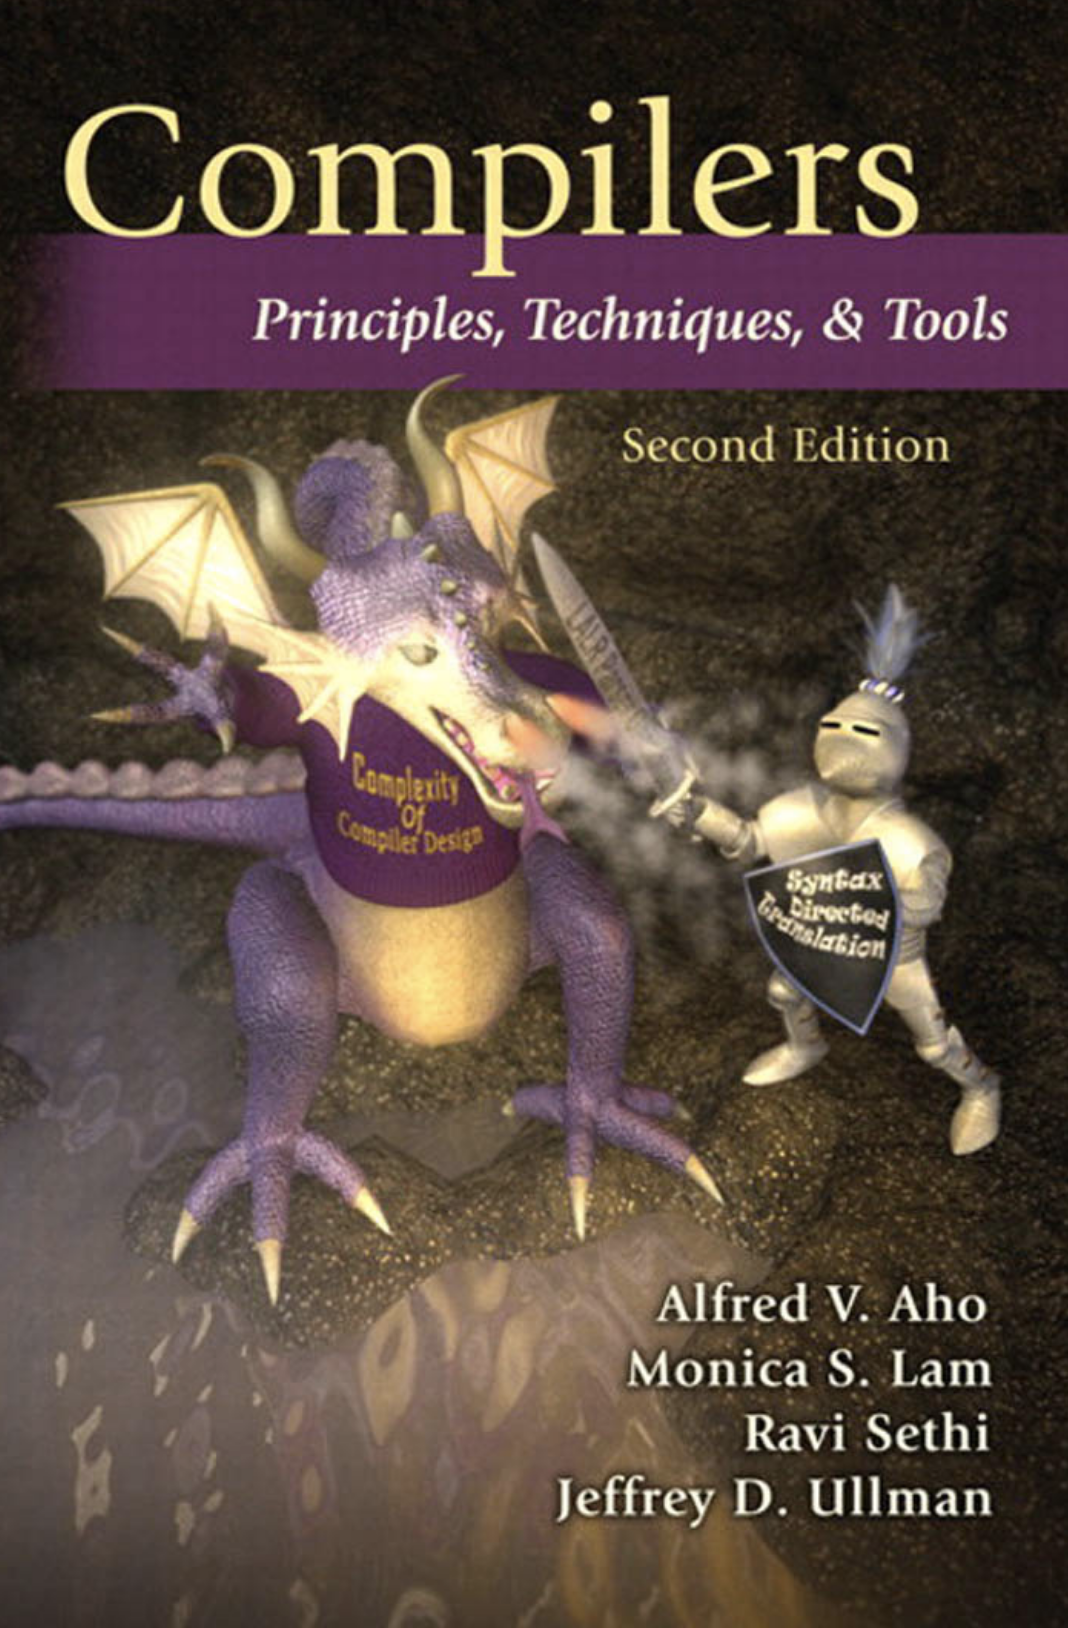
\includegraphics[width=\marginparwidth]{img/dragonbook.png}
    \emph{The Dragon Book}
    
\includegraphics[width=\marginparwidth]{img/llvmlogo.png}
    \emph{LLVM Logo}
}~\cite{dragonbook} where the authors introduce compilers through the process of transforming software.
\begin{quotation}
    [B]efore a program can be run, it first must be translated into a form in which it can be executed by a computer.

    The software systems that do this translation are called \emph{compilers}.
\end{quotation}
Hence we can visualize the action of a compiler as a sort of informal function.
\begin{figure}[ht]
    \centering
    \tikzset{
        frame/.style={
                draw,
                text width=6em,
                text centered,
                minimum height=4em,
                drop shadow,
                fill=orange!40,
                rounded corners,
            },
    }
    \begin{tikzpicture}[font=\sffamily, thick, node distance=4cm]
        \node[align=center] (pl) {Programming \\ Language};
        \node[frame, right of=pl] (compiler) {Compiler};
        \node[align=center, right of=compiler] (ml) {Machine \\ Language};

        \draw[-stealth] (pl) -- (compiler);
        \draw[-stealth] (compiler) -- (ml);
    \end{tikzpicture}
    \caption{Action of Compiler}\label{fig:compiler}
\end{figure}

The term compiler was coined by Grace Hopper in the early 1950's while working on a system that could translate symbolic mathematics into a machine language.
Initially Hopper was met with resistance for her new idea.
\begin{quotation}
    I had a running compiler, and nobody would touch it because, they carefully told me, computers could only do arithmetic; they could not do programs.
    It was a selling job to get people to try it.
    I think with any new idea, because people are allergic to change, you have to get out and sell the idea.
    \attrib{Grace Hopper 1952~\cite{hopperquote}}
\end{quotation}
In the end she succeeded in selling the idea and compilers became a ubiquitous piece of modern computing infrastructure.
Since Hopper coined the term the job of a compiler has grown enormously and now encompasses line reconstruction, preprocessing, lexical analysis, syntax analysis, semantic analysis, conversion to an \ac{IR}, optimization, target dependent optimizations, and finally code generation.
Thankfully we will not need to understand all of these parts, and the majority of this document will focus on \aclp{IR}, optimizations, and code generation.

\subsection{Examples of Compilers}
\begin{description}
    \item[Latex] While perhaps not very obvious, \LaTeX{} is indeed a compiler in the sense that it takes in code, and produces a lower level representation of what the user wants to typeset. Usually that comes in the form of postscript which is another programming language that is read by printers (hardware) to produce the requested document.
    \item[TensorFlow:] TensorFlow is a platform for machine learning that embodies the structure of a compiler very nicely. Indeed it has a front-end where the user builds their model, an optimizer that speeds up the model, and once it's ready the model can be brought to multiple backends (in browser, mobile, laptop). This is all even before we talk about TensorFlow Quantum which was introduced in~\cite{tensoflowquantum} to aid in optimizing noisy circuits on \acs{NISQ} devices.\footnote{We will get into, and define this terminology shortly!}
    \item[clang:] This \emph{is} a compiler in the strictest sense. As input it takes C/C++ and provides executable versions of that code that an be run on hardware.
\end{description}

\subsection{Intermediate Representations}

Suppose we have the following line in our code.
\begin{center}
    \verb|x_final = x_initial + velocity * time|
\end{center}
From this, one of the first steps the front end of a compiler might do is generate what's called a \textbf{syntax tree}.
This is a representation of the line of code in a tree format as in~\cref{fig:syntaxtree}.
While it may not be obvious why this is a helpful representation of the line of code, it \emph{is} indeed a representation that is used for further processing.
In this context, what we see in~\cref{fig:syntaxtree} is known as an \ac{IR} because it is not the initial, nor final representation of the piece of code.
While the compiler has the code in this state it can perform syntax and semantic analysis to ensure the code is well formed (syntactically), and meaningful (semantically).
Optimizations may also be performed.
\Eg{} if \verb|distance = velocity * time| has already been calculated, the subtree
\begin{figure}[htbp]
    \centering
    \Tree [.* velocity time]
    \caption{hi}
\end{figure}
can be replaced by simply \texttt{distance}.

\begin{figure}[ht!]
    \centering
    \newcommand{\qleafhook}[1]{\texttt{#1}}
    \newcommand{\qlabelhook}[1]{\texttt{#1}}
    \Tree [.= x\_final [.+ x\_initial [.* velocity time ] ] ]
    \caption{Syntax Tree}\label{fig:syntaxtree}
\end{figure}

\subsection{Computer Architecture}
To understand why it is we need compilers in the first place, we need to understand how modern computers work.
In a highly simplified model we can think of a computer as a \ac{CPU} connected to input and output devices (think keyboard and screen), and some sort of memory.
\begin{figure}[ht]
    \centering
    \tikzset{
        frame/.style={
                draw,
                text width=6em,
                text centered,
                minimum height=4em,
                drop shadow,
                fill=orange!40,
                rounded corners,
            },
        line/.style={
                draw, -latex',rounded corners=3mm,
            }
    }
    \begin{tikzpicture}[font=\sffamily, thick, node distance=4cm]
        \node[frame](input){Input Device(s)};
        \node[frame, below=2cm](output){Output Device(s)};
        \node[frame, below right=-.15cm and 1cm of input](cpu){CPU};
        \node[frame, right of=cpu](memory){Memory};

        \path[line] (input) -| (cpu);
        \path[line] (cpu) |- (output);
        \draw[stealth-stealth] (cpu) -- (memory);
    \end{tikzpicture}
    \caption{von Neumann Architecture scheme}\label{fig:comparch}
\end{figure}

At the very basic level, a \ac{CPU} has a finite number of possible operations it can perform despite there being a much larger input space of ``possible programs'' that we can feed it.
How then does the computer take a script and run it on it's \ac{CPU}?


Chris Lattner (the founder of one of the largest compiler projects; LLVM) has characterized compilers succinctly in~\cite{lattnerquote} as
\begin{quote}
    the art of allowing humans to think at a level of abstraction that they want to think about.
\end{quote}

\paragraph{Abstraction} With Lattner's quote in mind we can think of compilers as the tool that allows us to work with languages that are very abstract when compared to the instructions our \ac{CPU} can perform.
There also exist tools known as decompilers which take executables and turn them back into source code.
This operation is almost never the inverse of compiler because most languages allow for many ways of writing code that performs the same task.
With these tools we can raise and lower our levels of abstraction as desired and further push the details of the ``metal'' or hardware implementation away.


\section{LLVM}\label{sec:llvm}

% \subsection{\acf{MLIR}}
%*****************************************
\chapter{Quantum Computation}\label{ch:computation}
%*****************************************

In this chapter we will lay the groundwork for the necessary ideas from quantum computation.
We will not attempt to introduce quantum computation from the ground up, but instead introduce and emphasize some ideas we will focus on first.
The notation used here will mostly follow~\cite{watroustqi} and we recommend~\cite{nielsenchuang} for a more thorough introduction to the material.

\section{Historical Development}\label{sec:history}
Without a precise definition of quantum computing it's hard to give a precise storyline through the subject.
However, ideas rarely have clear cut boundaries and we must push forward to understand our messy world regardless.

One of the core tenets of quantum theory is that, at this scale, nature is reversible.
Hence when physicist Charles H. Bennett began investigating reversible Turing machines in~\cite{reversibleturing} we might say the field of quantum computing was \emph{just} beginning to start.
Since Turing machines are the mathematical and theoretical foundation for modern computers, it makes sense that a reversible Turing machine might lay the groundwork as the foundation for a computer that operators under quantum mechanical law.
More than 6 years later, Paul Benioff extended this work to describe a fully quantum mechanical version of a Turing machine in his paper \citetitle{quantumturing}~\cite{quantumturing}.

Once the theoretical foundation had been laid by Bennett and Benioff, Richard Feynman brought the idea mainstream when he proposed using these new computers to simulate quantum mechanics itself.
This idea was very attractive at the time (1981) since our classical computers were not powerful enough to simulate large quantum systems,\footnote{In fact, they still aren't!} and since Feynman was such a popular figure the idea finally took hold.
Feynman motivated the need for a new paradigm in computing as such:
\begin{quote}
    Nature isn't classical, dammit, and if you want to make a simulation of nature, you'd better make it quantum mechanical, and by golly it's a wonderful problem, because it doesn't look so easy.
    \attrib{Richard P. Feynman~\cite{feynmansimulator}}
\end{quote}

Even with one of the most famous physicists popularizing the idea, it took another 10 years to see the next major development which came in~\cite{deutch-jozsa-algo} where David Deutsch and Richard Jozsa gave an example of a problem that is solved exponentially faster on a quantum computer than a classical one.
If there was any hesitancy from the academic community at this point about the theoretical usefulness of a quantum computer, this result showed real potential for the emerging technology.
More applications start rolling in with quantum teleportation~\cite{quantumteleportation} and famously Peter Shor's polynomial time algorithm to factor integers (and hence break many modern cryptosystems)~\cite{shor-encryption}.

The latter caught the eye of the US Government and within the year of Shor's publication the \ac{NIST} organized the first government funded conference on quantum computation.\footnote{It's likely this is when quantum computation was put on the radar of the US government. In 2014 leaked documents showed the National Security Agency had begun a project dubbed ``Owning The Net'' whose purpose was to use a quantum computer to break internet cryptography and to ``gain access to and securely return high value target communications''. The status of the project---which also goes under the moniker ``Penetrating Hard Targets''---is unknown.}
There have been many major milestones since this, but perhaps most important to note is the first experimental realization of a qubit happened in~\citeyear{firstqubit} by Yasunobu Nakamura and Jaw-Shen Tsai~\cite{firstqubit}.
Hence it was less than 20 years from when Feynman demonstrated the potential usefulness of a quantum computer to the first experimental realization of the idea.

Since then ambitions have risen and technological progress has allowed for more and more qubits and quantum computers today have even been shown to complete tasks that classical ones cannot in any feasible amount of time.
In particular a team at China's Hefei National Laboratory used their 66-qubit computer\footnote{Affectionately named Zuchongzhi after Chinese mathematican Zu Chongzhi whose computation of $\pi$ was more accurate than any other for more than 800 years.} to complete a task in 4 hours that would take the most performant classical computers tens of thousands of years~\cite{zuchongzhi}.

More recently John Preskill has coined the term \ac{NISQ} as a characterization of the quantum computers that have dominated the past decade, and will likely continue to for the next few years~\cite{nisq}.
He takes these to be computers with 50--100 qubits for which noise will be a major factor in deciding what quantum circuits we can and cannot run.
The problem presented in this document is relevant to quantum computers past the \ac{NISQ}-era, but are especially important as we attempt to squeeze every ounce of computation out of them.

% TODO conclusion

\section{Quantum Computation}

In this section we will go over the basics of quantum computation.
% This section is written with a moderate amount of protest since I do not believe I will give a pedagogically proper and sound treatment of the material. % TODO make this a little lighter
Before continuing I would like to recommend~\cite{nielsenchuang} as well as \url{https://quantum.country} as great resources to learn the basics of quantum computing.

% TODO: talk about these
% There are three main models used for quantum computation:
% \begin{itemize}
%     \item circuital quantum computing
%     \item adiabatic quantum computing
%     \item measurement based quantum computing
% \end{itemize}
% Because of the ease in implementing universal quantum computation, the circuital model has become the most popular. % TODO

\subsection{Formalism}

A quantum bit, or \textbf{qubit} for short, is a vector $\ket{\psi}$ in 2-dimensional complex space $\C^2$ such that $\norm{\ket{\psi}} = 1$.
Often the following canonical basis is chosen and referred to as the computational basis.
\begin{align}
    \ket{0} \defeq \mqty[1 \\ 0] & & \ket{1} \defeq \mqty[0 \\ 1]
\end{align}
In this basis a qubit is a vector
\begin{equation}\label{eq:qubit}
    \ket{\psi} = \alpha\ket{0} + \beta\ket{1} = \mqty[\alpha \\ \beta]
\end{equation}
with the normalization condition that $\abs{\alpha}^2 + \abs{\beta}^2 = 1$.
In the case of \cref{eq:qubit} the state $\ket{\psi}$ is said to be in a \textbf{superposition} of state $\ket{0}$ and $\ket{1}$.

We often need to understand more complicated systems than just simple qubits, and to do so we use the \textbf{tensor product} to build up systems from subsystems.
\Eg{} if $\ket{\psi}\in\C^2$ and $\ket{\phi}\in\C^2$ represent two distinct physical qubits, we can represent the combined system as a single vector $\ket{\psi}\otimes \ket{\phi}$ in a larger complex Euclidean space $\C^2\otimes \C^2\cong \C^4$.
In the computational basis we can expand this as
\begin{align}
    \ket{\psi}\otimes \ket{\phi} & = \qty(\alpha\ket{0} + \beta\ket{1})\otimes\qty(\gamma\ket{0} + \delta\ket{1})                                                                \\
                                 & = \alpha\gamma\ket{0}\otimes\ket{0} + \alpha\delta\ket{0}\otimes\ket{1} + \beta\gamma\ket{1}\otimes\ket{0} + \beta\delta\ket{1}\otimes\ket{1}
\end{align}
where $\alpha, \beta, \gamma, \delta \in \C$.

With the objects of the theory defined, we must now understand the dynamics, or choreography of the theory.
As stated in~\cref{sec:history}, we take the theory of quantum mechanics to be reversible, and hence any operation we perform on a qubit $\ket{\psi}$ must be undo-able.
Thankfully linear algebra has just the tool to transform complex vectors in a reversible, and general way: unitary matrices!
\begin{definition}
    An $n\times n$ matrix $A$ is called \emph{unitary} if
    \begin{equation}\label{eq:unitary}
        AA^\dagger = A^\dagger A = \1
    \end{equation}
    where $^\dagger$ is the conjugate transpose.
    The collection of unitary matrices of dimension $n$ is called the \emph{unitary group} and is denoted \gls{un}.
\end{definition}
Hence when we have a qubit $\ket{\psi}$ and perform some action on it, we then have a new state $\ket{\phi} = U\ket{\psi}$ where $U$ represents whatever action we performed.
The condition shown in~\cref{eq:unitary} is quite restrictive: where a general $n \times n$ matrix has $2n^2$ real degrees of freedom, an element of $\U{n}$ only has $n^2$.\footnote{This is to say $\dim_\R\U{n} = n^2$.}
In fact for a general element of $\U{2}$ we can decompose it into pieces that look much more familiar.
\begin{example}
    Let $A$ be an arbitrary element of $\U{2}$.
    Then the following decomposition holds for $\alpha, \beta, \gamma, \delta \in \R$.
    \begin{equation}
        A = \e^{\iu\alpha}\mqty[\dmat[0]{\e^{-\iu \beta}, \e^{\iu \beta}}]\mqty[\cos\gamma & -\sin\gamma \\ \sin\gamma & \phantom{+}\cos\gamma]\mqty[\dmat[0]{\e^{-\iu \delta}, \e^{\iu \delta}}]
    \end{equation}
    As we can see the middle matrix is simply a 2D rotation matrix, and the other two are of a simple diagonal form.
    Lastly we have the global phase $\e^{\iu \alpha}$.
\end{example}

This is a particularly important example as the idea of decomposing unitary matrices into simpler pieces is something we will need heavily in circuit compilation tasks.
This decomposition also shows how attached to each unitary there is a phase ($\e^{\iu\alpha}$ in the above case), which in quantum computation is often irrelevant.
For that reason we also often work in the following group.
\begin{definition}
    If $A \in \U{n}$ be a unitary matrix that has the further property that
    \begin{equation}
        \det A = 1
    \end{equation}
    then $A$ is called a \emph{special unitary matrix} and we denote the collection of these matrices by $\gls{sun}$.
\end{definition}

\subsection{Quantum Gates}
A quantum gate is simply any unitary.
In this document we will mainly discuss quantum gates acting on 1 to 3 qubits since that is the range most quantum algorithms make use.
Most physical quantum computers today can perform single and double qubit gates.
\begin{table}[ht] % TODO make skinnier with text flow around?
    \centering
    % \begin{noindent}
    \begin{tabular}{cccc}
        Name           & Notation & Circuit Diagram                                                                                 & Matrix                                                 \\ \toprule
        Pauli X        & $X$      & \begin{tikzcd} \qw & \gate{X} & \qw \end{tikzcd}                                                & $\smqty[0 & 1 \\ 1 & 0]$                               \\
        Pauli Z        & $Z$      & \begin{tikzcd} \qw & \gate{Z} & \qw \end{tikzcd}                                                & $\smqty[1 & \phantom{-}0 \\ 0 & -1]$                   \\
        Hadamard       & $H$      & \begin{tikzcd} \qw & \gate{H} & \qw \end{tikzcd}                                                & $\frac{1}{\sqrt{2}}\smqty[1 & \phantom{-}1 \\ 1 & -1]$ \\
        Controlled Not & \CNOT    & \begin{tikzcd} \qw & \ctrl{1} & \qw \\ \qw & \targ{} & \qw \end{tikzcd}                         & $\smqty[1 & & & \\ & 1 & & \\ & & 0 & 1 \\ & & 1 & 0]$ \\
        Toffoli        & \CCNOT   & \begin{tikzcd} \qw & \ctrl{1} & \qw \\ \qw & \ctrl{1} & \qw \\ \qw & \targ{} & \qw \end{tikzcd} & $\smqty[1 & & & & & & & \\ & 1 & & & & & & \\ & & 1 & & & & & \\ & & & 1 & & & & \\ & & & & 1 & & & \\ & & & & & 1 & & \\ & & & & & & 0 & 1 \\ & & & & & & 1 & 0]$
    \end{tabular}
    % \end{noindent}
    \caption{Common Quantum Gates}\label{tab:commongates}
\end{table}


\begin{example}
    As we will later see, it is often important to be able to move qubits around on a physical chip.
    To do this we cannot physically move them, but rather apply some sort of combination of gates enact the swap.
    Thus we are looking for a unitary operation $\SWAP: \C^2\otimes \C^2 \to \C^2\otimes \C^2$ that acts as $\SWAP\qty[\ket{\psi}\otimes\ket{\phi}] = \ket{\phi}\otimes\ket{\psi}$.
    This is can be done using \CNOT{} gates and is shown diagrammatically.
    \begin{equation}\label{eq:cnotswap}
        \begin{quantikz}
            & \ctrl{1} & \targ{}   & \ctrl{1} & \midstick[2,brackets=none]{$\eqdef$} \qw & \swap{1} & \midstick[2,brackets=none]{$\equiv$} \qw & \gate[swap]{} & \qw \\
            & \targ{}  & \ctrl{-1} & \targ{}  & \qw                               & \targX{} & \qw                               &               & \qw
        \end{quantikz}
    \end{equation}
    Where the first equality shows us how to perform the swap with 3 \CNOT{} gates, and the last equality is an equivalence of notation.

    We can also show this using more mathematical notation if we understand the \CNOT{} map to act as $\CNOT\qty[\ket{x}\otimes\ket{y}] = \ket{x}\ket{x\oplus y}$ where $x, y \in \F$ and $\oplus$ is binary addition.
    With this we can explicitly compute the action of this circuit.
    Here we use the notation $\CNOT^a_b$ to mean a $\CNOT{}$ gate acting from qubit $a$ (the control qubit) to qubit $b$ (the target qubit).
    Then the 3 \CNOT{} gates in~\cref{eq:cnotswap} act under the following manipulations.
    \begin{align*}
        \ket{x}\otimes\ket{y} & \xrightarrow{\CNOT^1_2} \ket{x}\otimes\ket{x\oplus y}                                                     \\
                              & \xrightarrow{\CNOT^2_1} \ket{x\oplus (x\oplus y)}\otimes \ket{x\oplus y}  = \ket{y}\otimes\ket{x\oplus y} \\
                              & \xrightarrow{\CNOT^1_2} \ket{y}\otimes\ket{(x\oplus y)\oplus y} = \ket{y}\otimes \ket{x}.
    \end{align*}
    Thus exactly as desired.
\end{example}

\subsection{Quantum Circuits}

We are now ready to start putting these pieces together to build larger structures.
Since it is common that a quantum computer can perform a multitude of gates, we collect these together to form a \textbf{quantum gate set}.
These are the gates that we will be able to natively perform on our hardware.
\begin{definition}
    A \emph{quantum gate set} is a (typically finite) subset $G \subseteq \U{2^n}$. An element of $G$ is called a quantum gate.
\end{definition}
From these gates, we can construct a \textbf{quantum circuit} by applying a sequence of elements from the gate set.
\begin{definition}\label{def:circuit}
    Let $G$ be a quantum gate set, and let \gls{kleene} denote\footnote{This $^*$ operation is known as the Kleene star.} the set of finite length words over $G$ (and the empty word which we take to mean identity).
    A \emph{quantum circuit} is an element of $G^*$.
\end{definition}
Thus if our gate set $G = \qty{a, b, c}$, then some example circuits may be $aacba$, $cccbbb$, $cbbbab$, and $ab$.

Something to note here is that in this abstraction, all of our quantum gates are assumed to act on all qubits.
Hence, with a 2 qubit quantum chip and the ability to perform a Pauli $X$ gate on either qubit, then our gate is $\qty{\1\otimes \1, \1\otimes X, X\otimes \1, X\otimes X}$.\footnote{We don't always think of the identity gate $\1$ as a gate that needs to be included, but doing nothing to a qubit is no easy task, so it's important to remember to treat it just like any other gate and understand it's error rates as well.}
Sometimes this gate set is denoted $\qty{\1, X_0, X_1, X_0X_1}$, but we will try to use more explicit notation here.

Circuits are often drawn using diagram as in~\cref{fig:excircuit} where each horizontal ``wire'' represents a qubit, and boxes and other gadgets represent quantum gates.
\begin{figure}[ht]
    \centering
    \begin{quantikz}
        & \gate{U_0} & \ctrl{1} & \gate{U_1} & \ctrl{1}            & \qw           & \gate[wires=3]{U_3} & \qw \\
        & \gate{U_0} & \targ{}  & \qw        & \gate[wires=2]{U_2} & \gate[swap]{} &                     & \qw \\
        & \gate{U_0} & \qw      & \qw        &                     &               &                     & \qw
    \end{quantikz}
    \caption{Example Quantum Circuit}\label{fig:excircuit}
\end{figure}
That said, the way our theoretical model sees this circuit is more like that of~\cref{fig:abstractcircuit} where each gate acts on the entirety of the qubits.
\begin{figure}[ht]
    \centering
    \begin{quantikz}
        & \gate[wires=3][0.8cm]{A} & \gate[wires=3][0.8cm]{B} & \gate[wires=3][0.8cm]{C} & \gate[wires=3][0.8cm]{D} & \gate[wires=3][0.8cm]{E} & \gate[wires=3][0.8cm]{F} & \qw \\
        &                   &                   &                   &                   &                   &                   & \qw \\
        &                   &                   &                   &                   &                   &                   & \qw
    \end{quantikz}
    \caption{Abstract Quantum Circuit}\label{fig:abstractcircuit}
\end{figure}
In~\cref{tab:gates2circuit} we see what each one of these circuits are under the hood, and we can know that all of them are in the gate set for the above circuit.
\begin{table}[ht]
    \centering\begin{tabular}{cc}
        Gate Name & Composition                   \\ \toprule
        $A$       & $U_0 \otimes U_0 \otimes U_0$ \\
        $B$       & $\CNOT \otimes \1$            \\
        $C$       & $U_1 \otimes \1 \otimes \1$   \\
        $D$       & $\controlled{U_2}$            \\
        $E$       & $\1 \otimes \SWAP$            \\
        $F$       & $U_3$                         \\
    \end{tabular}
    \caption{Gate Compositions}\label{tab:gates2circuit}
\end{table}

We now have the machinery for circuits, and one of the important questions we need to ask is \emph{when are two circuits the same?}
Surely we can compare the circuits as strings in $G^*$, but if $G = \qty{\1, X}$, it will not tell us that $C = \1$ and $C' = XX$ are the same despite the same physical process happening.
To this end we wish to understand how the combinations of gates come together to form the entire process.
Following~\cite{formalcircuit} we define a map $\dbrackets{-}: G^* \to \U{2^n}$ which takes a quantum circuit, or sequence of gates, and multiplies them together to obtain a single unitary operator: $\dbrackets{g_1g_2\cdots g_m} = g_m\cdot g_{m-1} \cdots g_1$.\footnote{Notice here on the left we have string concatenation, and on the right matrix multiplication. Also note the fact that when doing the multiplication we reverse the order. This is an artifact of the way we draw quantum circuits from left to write, but apply gates mathematically right to left.}
Then we can say two circuits $C$ and $C'$ are effectively the same if $\dbrackets{C} = \dbrackets{C'}$.

This formalism also allows us to frame the following important question about unitary synthesis.
\begin{question}\label{qu:synthesis}
    Given a quantum gate set $G$, and unitary operator $U\in\U{2^n}$, does there exist a circuit $C\in G^*$, such that $\dbrackets{C} = U$?
\end{question}
If the answer is yes, we say a gate set $G$ \textbf{synthesizes} $U$.
This question is answered, at least in part through the Solovay-Kitaev theorem first published in~\cite{bigkitaev} with further proofs/elucidations in~\cite{nielsenchuang,solovay-kitaev,kitaev-book}.
The theorem, stated in our terminology follows.
\begin{theorem}[Solovay-Kitaev]\label{thm:solovaykitaev}
    Let $G$ be a quantum gate set such that
    \begin{itemize}
        \item $g\in\SU{2^n}$ for all $g\in G$,
        \item $g^\dagger \in G$ for all $g\in G$, and
        \item the free group $\free{G}$ is dense in $\SU{2^n}$.
    \end{itemize}
    Take $\varepsilon > 0$.
    Then, there is a constant $c > 3$, such that for any $U\in\SU{2^n}$, there exists a circuit $C\in G^*$ of length $\order{\log^c\qty(\frac{1}{\varepsilon})}$ that approximates $U$: that is $\norm{\dbrackets{C} - U} < \varepsilon$. % TODO: a lot of undefined stuff here \norm, \order (assumed, but not stated), free group
\end{theorem}
Not only does this theoretical result provide some insight into~\ref{qu:synthesis}, but it's constructive and hence provides an algorithm\footnote{This result sometimes goes under the name ``The Solovay-Kitaev Algorithm''.} to approximate arbitrary elements of $\SU{2^n}$ using gates from $\SU{2^m}$ for any $m \in \gls{intsn}$.
This result was an important and motivating because it showed that one only need a finite number of gates to perform any unitary.

With at least a partial answer to Question~\ref{qu:synthesis} we can begin to refine further questions.
If the answer to~\ref{qu:synthesis} is positive, we can then ask the following.
\begin{question}\label{qu:optimalsynthesis}
    If $G$ synthesizes $U$, and if $f: G^* \to \R$ is a cost function, can we find
    \begin{equation*}
        C_\text{min} = \argmin_{C\in G^*} \qty{f(C) : \dbrackets{C} = U}?
    \end{equation*}
\end{question}
Some examples of common cost functions are given below, and multiple can be used in the case of tie-breaking.
\begin{itemize}
    \item $f(C) = \mathtt{length}(C)$ (commonly referred to as the depth of the circuit)
    \item $f(C) = $ \# of uses of a particular gate in $C$
    \item $f(C) = \mathtt{duration}(C)$ (by this we mean the total elapsed time the circuit takes)\footnote{We have not discussed this yet, but each gate $g\in C$ takes a nonzero amount of time, during which the computation may be disturbed by outside forces.}
\end{itemize}

\subsection{Universal Gate Sets}\label{sec:universal}

We slightly danced around the idea of universality in~\cref{thm:solovaykitaev}, but we will make it clear now.
In order to harness the full power of a quantum computer, we hope it to be able to perform arbitrary unitary operations.
\begin{definition}
    A gate set $G$ on $n$ qubits is called \emph{universal} if for all $U\in\U{2^n}$ there exists a circuit $C\in G^*$ such that $\dbrackets{C} = U$.
\end{definition}
If our gate set is not universal, then we can often find ourselves in a situation where it is more efficient to simulate a given quantum algorithm than to actually run it.
\Eg{} circuits composed of gates from $\qty{\CNOT, H, S}$ are known to be efficiently simulable~\cite{gottesman-knill} despite not limiting factors typically thought to make quantum computation more powerful such as entanglement.

The question of which gate sets are universal for quantum computation is important both for our theoretical understanding of quantum computation, but also for building physical devices.
Examples that have been shown to be universal are
\begin{itemize}
    \item \CNOT{} plus $\U{2}$ as shown in~\cite{universal-cnot-u2}
    \item \CNOT{}, Hadamard, and the $\frac{\pi}{8}$-gate\footnote{The $\frac{\pi}{8}$-gate is also sometimes called $T$ and has matrix representation $\smqty[1 & 0 \\ 0 & \e^{\iu\pi/4}]$.} as shown in~\cite{universal-cnot-had-p8}
    \item \CCNOT{} (Toffoli), Hadamard, and the $\frac{\pi}{4}$-gate\footnote{The $\frac{\pi}{4}$-gate is also sometimes called $S$ and has matrix representation $\smqty[1 & 0 \\ 0 & \e^{\iu\pi/2}]$.} as shown in~\cite{bigkitaev}
    \item \CNOT{} plus any single qubit gate that does not preserve the computational basis and is not the Hadamard gate as shown in~\cite{universal-cnot-basis-change}
\end{itemize}

\section{Mathematics} % TODO cover some math for solovay-kitaev

Before moving on there are a few more bits of mathematics we need to cover.
All of our discussions in this section will assume our vector space $V$ is some complex space $\C^n$.

\subsection{Operator Norms}

\paragraph{Vector induced norms:}
Suppose our vector space $V$ has an existing norm defined on it $\norm{\cdot}: V \to \R$.
This induces a norm on the space of operators \gls{endV} as
\begin{equation}
    \norm{A}_\text{vec} \defeq \max_{v \in V}\qty{\norm{A v}: \norm{v} = 1}.
\end{equation}

\paragraph{Trace norm:}
\begin{equation}
    \norm{A}_\text{tr} \defeq \tr(\sqrt{A^\dagger A})
\end{equation}

\paragraph{Frobenius norm:}
\begin{equation}
    \norm{A}_\text{F} \defeq \sqrt{\tr(A^\dagger A)} = \qty(\sum_{i, j \in [n]}\abs{a_{ij}}^2)^{1/2} = \norm{\vectorize(A)}
\end{equation}


\subsection{Free Group}
We will not attempt a rigorous definition of the free group and instead opt for something more informal since we will not need to work with the details.
Let $S$ be a finite set, and denote by $S^{-1}$ the formal inverse of elements in $S$.
Then the free group $\free{S} \defeq (S\cup S^{-1})^*$ where the asterisk indicates the Kleene star.

As an example take $S = \qty{f, g, h}$, and hence $S^{-1} = \qty{f^{-1}, g^{-1}, h^{-1}}$.
Then the free group $\free{S}$ contains elements such as $fg^{-1}hhhh^{-1}$, $fghhhf$, and $h^{-1}gh^{-1}f^{-1}ghgg$.
Note that this may appear very similar to~\cref{def:circuit}, however we did not require our ``words'' to be over the inverses as we have here; only elements of the set itself.\footnote{This is done because in practice, being able to perform a quantum gate $U$, does not always imply we can easily perform it's inverse $U^\dagger$.} % TODO: cref not working properly with named stuff

\subsection{Dense-ness}

What does it mean for a gate set $G$ to be dense in $\SU{2^n}$?
It means that for every $U \in \SU{2^n}$, and every $\varepsilon > 0$, we have a sequence of gates $C = g_1g_2\cdots g_m$ such that $\norm{\dbrackets{C} - U} < \varepsilon$.

\subsection{Fidelity}

Suppose $\rho$ and $\sigma$ are two density operators.
Their \textbf{fidelity} is a measure of how similar the two states are and is given by
\begin{equation}
    \Fid(\rho, \sigma) \defeq \norm{\sqrt{\rho}\sqrt{\sigma}}_\text{tr} = \tr(\sqrt{\sqrt{\sigma}\rho\sqrt{\sigma}}).
\end{equation}
We can see if $\rho = \sigma$, then their fidelity is equal to 1, and otherwise this value lies between 0 and 1.
This notion can be expanded from quantum states to quantum gates to obtain a measure of how well one unitary approximates another~\cite{fidelity}.
Since $\Fid(\rho, \sigma)$ is a measure of distance between states $\rho$ and $\sigma$, and we are interested in understanding the difference of a quantum circuit and a specified target unitary, then we can calculate $\Fid(U\rho U^\dagger, \mathcal{E}(\rho))$.\footnote{Here we are using $\mathcal{E}$ to denote some quantum circuit, and $\mathcal{E}(\rho)$ it's action on $\rho$.}\todo{maybe change this notation.}
This is great, however to study a circuit more effectively, we'd like to ditch the associated state $\rho$ since we don't want to perform this analysis for every such $\rho$.
We can then define the \textbf{average gate fidelity} of a unitary $U$ and quantum circuit $\mathcal{E}$ as
\begin{equation}
    \Fid_\text{gate}(U, \mathcal{E}) \defeq \int \Fid(U\rho U^\dagger, \mathcal{E}(\rho))\dd{\rho}
\end{equation}
where the integral $\int\dd{\rho}$ is taken over all density operators.\todo{is this even right?}




\cleardoublepage

\ctparttext{
    The goal of this part is to familiarize the reader with the realities of quantum hardware.
    This means understanding their architecture, strengths, weaknesses, and some of the many measures we have to quanitify their effectiveness.
    With an understanding of the limitations of hardware we can decisively understand the problem of quantum circuit compilation.
    We will show how the problem is both similar and different from classical compilation and how we can benefit from using existing classical infrastructure.
}
\part{Back End}\label{part:backend}
%************************************************
\chapter{Quantum Hardware}\label{ch:hardware}
%************************************************

In this chapter we will give a brief overview of the necessary ideas one needs in order to understand the qubit mapping problem.

\section{Quantum Chips}

\begin{definition}
    A \emph{quantum chip's topology} is a graph $G = (V, E)$ with the vertices representing qubits, and edges representing connections between qubits where quantum gates of the correct arity can be applied.
\end{definition}

As an example take the the topology of IBM's \texttt{ibmq\_jakarta} shown in~\ref{fig:ibm-jakarta}.
``3'' being connected to ``1'' means that we can apply a 2-qubit unitary targeting both of those qubits, however the hardware does not support native 2-qubit gates between qubits ``2'' and ``6''.
\begin{figure}[ht]
    \centering
    \begin{tikzpicture}
        \tikzset{
            node/.style={
                    very thick,
                    circle,
                    fill=blue!20,
                    draw,
                    minimum size=.8cm,
                }
        }
        \node[node] (0) {$0$};
        \node[node] (1) [right = .8cm of 0] {$1$};
        \node[node] (2) [right = .8cm of 1] {$2$};
        \node[node] (3) [below = .8cm of 1] {$3$};
        \node[node] (5) [below = .8cm of 3] {$5$};
        \node[node] (4) [left  = .8cm of 5] {$4$};
        \node[node] (6) [right = .8cm of 5] {$6$};

        \path[draw, very thick]
        (0) edge node {} (1)
        (1) edge node {} (2)
        (1) edge node {} (3)
        (3) edge node {} (5)
        (5) edge node {} (4)
        (5) edge node {} (6);
    \end{tikzpicture}
    \caption{IBMQ Jakarta Architecture}\label{fig:ibm-jakarta}
\end{figure}

We can now define the main problem of quantum circuit compilation: that of the qubit mapping problem.\footnote{This sometimes also goes by the name of the qubit routing problem, or qubit scheduling problem although sometimes these mean slightly different things.}
If we have both a quantum circuit $C\in G^*$, and a quantum computer with network topology $G$, can the computer perform our circuit?
In order to address this question we must first talk about universal gate sets.

% In \cite{optimalSyn}
\section{T1}
\section{T2}
\section{CLOPS}


\section{Quantum Compilers}
We can now return to the issue of compilers.
It should now be clear that the level of abstraction we work at when designing quantum algorithms is much higher than the capabilities of our current, and likely future hardware.
Hence quantum compilers are needed for two steps.
\begin{figure}[h]
    \centering
    \tikzset{
        frame/.style={
                draw,
                text width=6em,
                text centered,
                minimum height=4em,
                drop shadow,
                fill=orange!40,
                rounded corners,
            },
    }
    \begin{tikzpicture}[font=\sffamily, very thick, node distance=4cm]
        \node[align=center] (qa) {Quantum \\ Algorithm};
        % \node[frame, right of=qa] (compiler) {Compiler};
        \node[frame, right of=qa] (ir) {};%Intermediate \\ Representation};
        \node[align=center, above right=.5cm and 1cm of ir] (ha) {Hardware A};
        \node[align=center, below=.5cm of ha] (hb) {Hardware B};
        \node[align=center, below=.1cm of hb] (hdots) {\vdots};

        % \node[align=center, right of=compiler] (ml) {Hardware A};

        \draw[-stealth] (qa) -- (ir);
        \draw[-stealth] (ir) -- (ha);
        \draw[-stealth] (ir) -- (hb);
        % \draw[-stealth] (ir) -- (hdots);

        \node[very thick, draw=orange!20, fit=(ir), inner sep=3mm, label=above:{Quantum Compiler}, rounded corners](qcompiler) {};
    \end{tikzpicture}
    \caption{Action of Quantum Compiler}\label{fig:quantumcompiler}
\end{figure}

% ***********************************************
\chapter{Quantum Compilers}\label{ch:qcomps}
% ***********************************************

We can now return to the issue of compilers.
It should now be clear that the level of abstraction we work at when designing quantum algorithms is much higher than the capabilities of our current, and likely future hardware.
Hence quantum compilers are needed for two steps.
\begin{figure}[h]
    \centering
    \tikzset{
        frame/.style={
                draw,
                text width=6em,
                text centered,
                minimum height=4em,
                drop shadow,
                fill=orange!40,
                rounded corners,
            },
    }
    \begin{tikzpicture}[font=\sffamily, very thick, node distance=4cm]
        \node[align=center] (qa) {Quantum \\ Algorithm};
        % \node[frame, right of=qa] (compiler) {Compiler};
        \node[frame, right of=qa] (ir) {};%Intermediate \\ Representation};
        \node[align=center, above right=.5cm and 1cm of ir] (ha) {Hardware A};
        \node[align=center, below=.5cm of ha] (hb) {Hardware B};
        \node[align=center, below=.1cm of hb] (hdots) {\vdots};

        % \node[align=center, right of=compiler] (ml) {Hardware A};

        \draw[-stealth] (qa) -- (ir);
        \draw[-stealth] (ir) -- (ha);
        \draw[-stealth] (ir) -- (hb);
        % \draw[-stealth] (ir) -- (hdots);

        \node[very thick, draw=orange!20, fit=(ir), inner sep=3mm, label=above:{Quantum Compiler}, rounded corners](qcompiler) {};
    \end{tikzpicture}
    \caption{Action of Quantum Compiler}\label{fig:quantumcompiler}
\end{figure}

\dots Thus when compiling circuits, we need to minimize the number of \SWAP{} gates we must add since we saw in~\cref{eq:cnotswap} that each \SWAP{} takes 3 \CNOT{} gates.

\paragraph{Compiling the Toffoli Gate}
Since most hardware are not capable of 3-qubit operations we must decompose the Toffoli, or \CCNOT{} gate into something more manageable.
This is typically done using \CNOT{}'s, Hadamard's ($H$), and $\pi/8$ ($T$) gates~\cite{nielsenchuang}.
\begin{equation}
    \begin{quantikz}[column sep=.25cm]
        & \ctrl{1} & \midstick[3,brackets=none]{$=$} \qw & \qw      & \qw      & \qw              & \ctrl{2} & \qw      & \qw      & \qw              & \ctrl{2} & \qw      & \ctrl{1} & \gate{T}         & \ctrl{1} & \qw \\
        & \ctrl{1} & \qw                                 & \qw      & \ctrl{1} & \qw              & \qw      & \qw      & \ctrl{1} & \qw              & \qw      & \gate{T} & \targ{}  & \gate{T^\dagger} & \targ{}  & \qw \\
        & \targ{}  & \qw                                 & \gate{H} & \targ{}  & \gate{T^\dagger} & \targ{}  & \gate{T} & \targ{}  & \gate{T^\dagger} & \targ{}  & \gate{T} & \gate{H} & \qw              & \qw      & \qw
    \end{quantikz}
\end{equation}
This is an important decomposition as the \CCNOT{} gate appears in the modular exponentiation problem which is a core part of Shor's algorithm~\cite{shor-encryption}.
Hence if there are smaller decompositions than shown above that would be ideal as \emph{one} \CCNOT{} gate becomes 14!
\citeauthor{universal-cnot-u2} show a more compact decomposition of \CCNOT{} using only 3 \CNOT{} gates if the phase of one of the qubits is allowed to change~\cite{universal-cnot-u2}.
Let $G = R_Y(\frac{\pi}{4})$ in the following circuit. % following https://arxiv.org/pdf/quant-ph/9705009.pdf rather than original paper
\begin{equation}
    \begin{quantikz}%[column sep=.25cm]
        & \ctrl{1} & \midstick[3,brackets=none]{$\approx$} \qw & \qw                        & \qw      & \qw                        & \ctrl{2} & \qw                       & \qw      & \qw                       & \qw \\
        & \ctrl{1} & \qw                                       & \qw                        & \ctrl{1} & \qw                        & \qw      & \qw                       & \ctrl{1} & \qw                       & \qw \\
        & \targ{}  & \qw                                       & \gate{G^\dagger} & \targ{}  & \gate{G^\dagger} & \targ{}  & \gate{G} & \targ{}  & \gate{G} & \qw
    \end{quantikz}
\end{equation}
However the question ended in~\citeyear{toff3cnot} when it was shown that a true equality preserving decomposition of the \CCNOT{} gate requires a minimum of 6 \CNOT{} gates~\cite{toff3cnot}.\footnote{This result shows that a minimum of 6 \CNOT{} gates must be used, \textbf{if} they are being used. Other decompositions not using \CNOT{} gates might still be more compact.}

\section{Strong and Weak Compilation}

\section{Compiling on a ring}

\section{Methods}

\section{Quantum Stack}


% ******************************************************
% Back matter
% ******************************************************
% \appendix
% \renewcommand{\thechapter}{\alph{chapter}}
% \cleardoublepage
% \part{Appendix}
% %********************************************************************
% Appendix
%*******************************************************
% If problems with the headers: get headings in appendix etc. right
%\markboth{\spacedlowsmallcaps{Appendix}}{\spacedlowsmallcaps{Appendix}}
\chapter{Appendix Test}
Lorem ipsum at nusquam appellantur his, ut eos erant homero
concludaturque. Albucius appellantur deterruisset id eam, vivendum
partiendo dissentiet ei ius. Vis melius facilisis ea, sea id convenire
referrentur, takimata adolescens ex duo. Ei harum argumentum per. Eam
vidit exerci appetere ad, ut vel zzril intellegam interpretaris.
\graffito{More dummy text.}

%Errem omnium ea per, pro congue populo ornatus cu, ex qui dicant
%nemore melius. No pri diam iriure euismod. Graecis eleifend
%appellantur quo id. Id corpora inimicus nam, facer nonummy ne pro,
%kasd repudiandae ei mei. Mea menandri mediocrem dissentiet cu, ex
%nominati imperdiet nec, sea odio duis vocent ei. Tempor everti
%appareat cu ius, ridens audiam an qui, aliquid admodum conceptam ne
%qui. Vis ea melius nostrum, mel alienum euripidis eu.

\section{Appendix Section Test}
Test: \autoref{tab:moreexample} (This reference should have a
lowercase, small caps \spacedlowsmallcaps{A} if the option
\texttt{floatperchapter} is activated, just as in the table itself
 $\rightarrow$ however, this does not work at the moment.)

\begin{table}[h]
    \myfloatalign
    \begin{tabularx}{\textwidth}{Xll} \toprule
        \tableheadline{labitur bonorum pri no} & \tableheadline{que vista}
        & \tableheadline{human} \\ \midrule
        fastidii ea ius & germano &  demonstratea \\
        suscipit instructior & titulo & personas \\
        %postulant quo & westeuropee & sanctificatec \\
        \midrule
        quaestio philosophia & facto & demonstrated \\
        %autem vulputate ex & parola & romanic \\
        %usu mucius iisque & studio & sanctificatef \\
        \bottomrule
    \end{tabularx}
    \caption[Autem usu id]{Autem usu id.}
    \label{tab:moreexample}
\end{table}

%Nulla fastidii ea ius, exerci suscipit instructior te nam, in ullum
%postulant quo. Congue quaestio philosophia his at, sea odio autem
%vulputate ex. Cu usu mucius iisque voluptua. Sit maiorum propriae at,
%ea cum primis intellegat. Hinc cotidieque reprehendunt eu nec. Autem
%timeam deleniti usu id, in nec nibh altera.




\section{Another Appendix Section Test}
Equidem detraxit cu nam, vix eu delenit periculis. Eos ut vero
constituto, no vidit propriae complectitur sea. Diceret nonummy in
has, no qui eligendi recteque consetetur. Mel eu dictas suscipiantur,
et sed placerat oporteat. At ipsum electram mei, ad aeque atomorum
mea. There is also a useless Pascal listing below: \autoref{lst:useless}.

\begin{lstlisting}[float=b,language=Pascal,frame=tb,caption={A floating example (\texttt{listings} manual)},label=lst:useless]
for i:=maxint downto 0 do
begin
{ do nothing }
end;
\end{lstlisting}

%Ei solet nemore consectetuer nam. Ad eam porro impetus, te choro omnes
%evertitur mel. Molestie conclusionemque vel at, no qui omittam
%expetenda efficiendi. Eu quo nobis offendit, verterem scriptorem ne
%vix.


% ******************************************************
% Other Stuff in the Back
% ******************************************************
\cleardoublepage% ******************************************************
% Bibliography
% ******************************************************
% work-around to have small caps also here in the headline
% https://tex.stackexchange.com/questions/188126/wrong-header-in-bibliography-classicthesis
% Thanks to Enrico Gregorio
\defbibheading{bibintoc}[\bibname]{%
  \phantomsection
  \manualmark
  \markboth{\spacedlowsmallcaps{#1}}{\spacedlowsmallcaps{#1}}%
  \addtocontents{toc}{\protect\vspace{\beforebibskip}}%
  \addcontentsline{toc}{chapter}{\tocEntry{#1}}%
  \chapter*{#1}%
}
\printbibliography[heading=bibintoc]

\cleardoublepage%*******************************************************
% Declaration
%*******************************************************
\pdfbookmark[0]{Declaration}{declaration}
\chapter*{Declaration}
\thispagestyle{empty}
This thesis consists of material all of which I authored.

I understand that my thesis may be made electronically available to the public.
\bigskip

\noindent\textit{\myLocation, \myTime}

\smallskip

\begin{flushright}
    \begin{tabular}{m{5cm}}
        \\ \midrule
        \centering\myName{} \\
    \end{tabular}
\end{flushright}

\cleardoublepage\pagestyle{empty}

\hfill

\vfill

\pdfbookmark[0]{Colophon}{colophon}
\section*{Colophon}
This document was typeset using the typographical look-and-feel \texttt{classicthesis} developed by Andr\'e Miede and Ivo Pletikosić.
The style was inspired by Robert Bringhurst's seminal book on typography ``\emph{The Elements of Typographic Style}''.
\texttt{classicthesis} is available for both \LaTeX\ and \mLyX:
\begin{center}
    \url{https://bitbucket.org/amiede/classicthesis/}
\end{center}

\bigskip

\noindent\finalVersionString

Hermann Zapf's \emph{Palatino} and \emph{Euler} type faces are used and the ``typewriter'' text is typeset in \emph{Bera Mono}.


\end{document}
